\documentclass[11pt]{report}

\usepackage{graphicx}
\usepackage{caption}

\marginparwidth 0.5in 
\oddsidemargin 0.25in 
\evensidemargin 0.25in 
\marginparsep 0.25in
\topmargin 0.0in 
\textwidth 6in \textheight 8.5in

\title{sQuire: A Web Based Collaborative Editor\\Class Diagrams\\Group 3}
\author{Rick Boss (boss2849)}

\begin{document}
\maketitle

\newpage

\section{Compiler (boss2849)}
    \begin{minipage}{1\textwidth}
        \begin{center}
            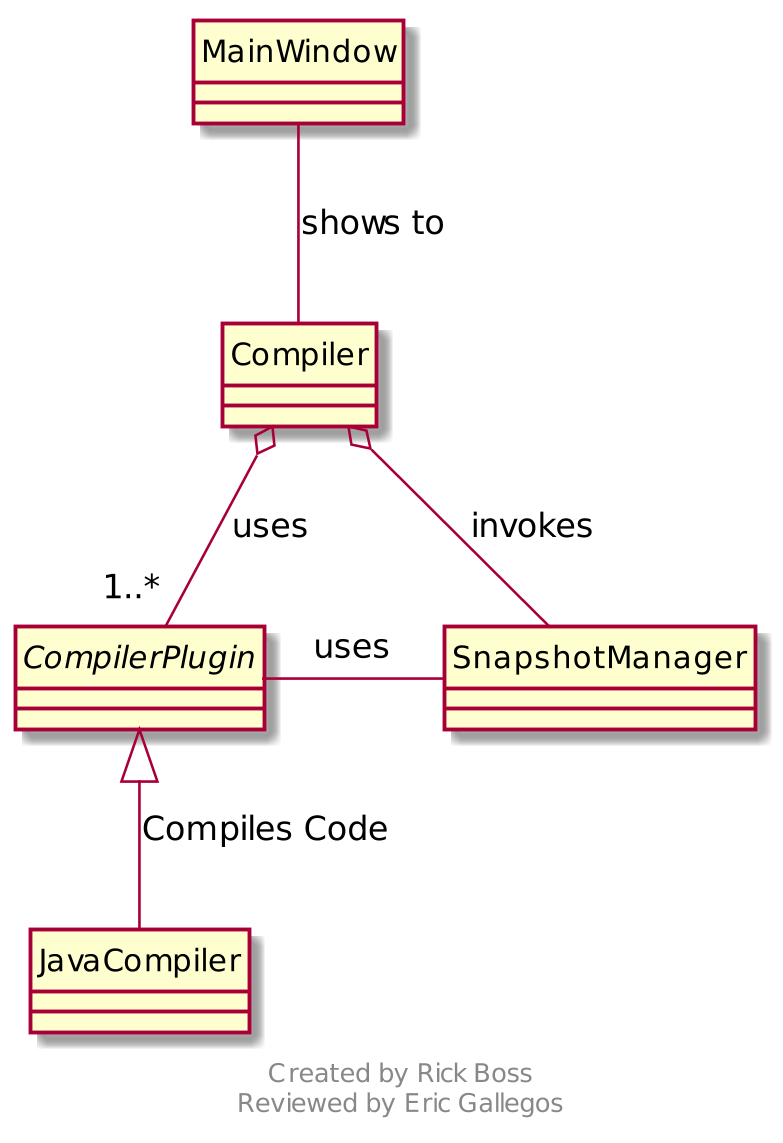
\includegraphics[width=0.7\textwidth]{compiler-boss2849}
        \end{center}
        \captionof{figure}{The Compiler is invoked from the main window. From here, the Compiler will select the appropriate CompilerPlugin determined by the configured compiler for the project. The compiler also invokes the SnapshotManager, which stores the current state of the code to be used during compilation. In this simple example, only a JavaCompiler plugin is present, but there can be more than one plugins available in the future. The JavaCompiler plugin retrieves the code snapshot from the SnapshotManager and compiles the code.}
    \end{minipage}

\end{document}
